\documentclass[thesis.tex]{subfiles}

\begin{document}
\chapter{Results}
The approach to the unification of CoBundleMAP and FBA analysis for the extension of the resulting feature vector, described in the Method chapter, was successfully implemented. Several runs of resulting pipeline were performed with different parameters and techniques of the population template generation. Achieved results were visualized, corresponding plots and their discussion is presented within this chapter.

The population that was used within this thesis consists of 19 subjects with differing manifestations of hippocampal sclerosis -- a neurological condition closely related to temporal lobe epilepsy and characterized by neuronal loss and gliosis. The subjects were classified in one of the three groups, depending on the hemisphere affected by the disease, resulting in 10 "Left" class, 7 "Right" class, and 2 "Left-and-right" class patients.

Analysis was performed on a set of 16 white matter bundles (each bundle being split into right and left parts) -- \textit{anterior thalamic radiation} (ATR), \textit{cingulum} (CING), \textit{cortispinal tract} (CST), \textit{fornix} (FORN), \textit{inferior fronto-occipital fasciculus} (IFO), \textit{inferior longitudinal fasciculus} (ILF), \textit{superior longitudinal fasciculus} (SLF), and \textit{ventral tegmental area} (VTA).

Visualizations presented in this chapter were performed by splitting the samples into two distinct groups, representing affected and healthy hemispheres.

\begin{figure}[tbh!]
	\begin{minipage}[b]{0.49\linewidth}
		\centering
		\centerline{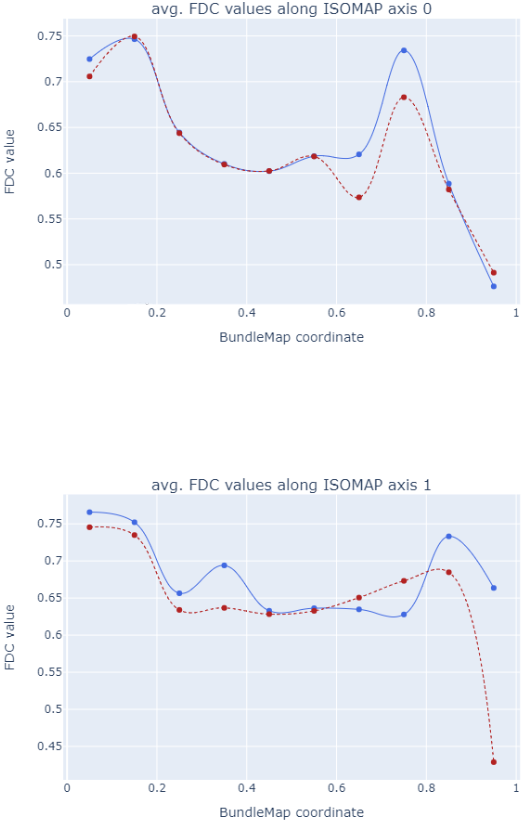
\includegraphics[width=7.3cm]{thesis_radomskyi/images/first-ifo-no-ups.png}}
		\centerline{(a) Without upsampling}\medskip
	\end{minipage}
	\hfill
	\begin{minipage}[b]{0.49\linewidth}
		\centering
		\centerline{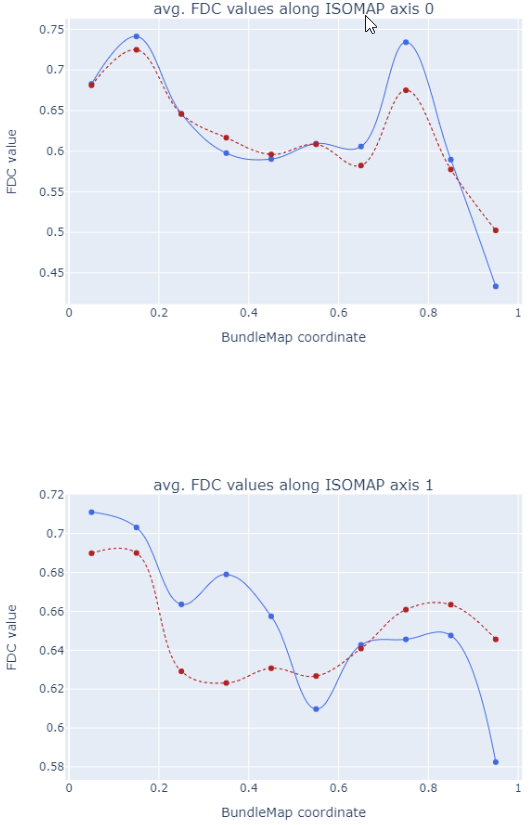
\includegraphics[width=7.3cm]{thesis_radomskyi/images/first-ifo-with-ups.png}}
		\centerline{(b) With upsampling}\medskip
	\end{minipage}
	\caption{\textbf{Results for IFO bundle with upsampling.}}
  \label{fig:first-ifo}
\end{figure}

As mentioned above, computation of population template for the FBA analysis was performed using different techniques. One of such methods is upsampling -- increasing of resolution, performed by resizing the image voxels. Upsampling was performed to a voxel size of 1.3 mm and compared with original dimensionality of approximately 1.7 mm. The difference in achieved results can be neglected, since correlations are equally visible on both, as observed from results for IFO bundle, presented at Figure \ref{fig:first-ifo}. Though increase in dimensionality is considered to be an important step of FBA analysis, and is reported to produce more robust results due to additional detalization and better alignment of fixel directions, the data that I worked with seems to be too well-processed for this to affect the results in any considerable way. Nevertheless, I will be using parameterizations acquired from the upsampled population, since the resulting bundles have less abnormalities at the ends (e.g. empty bins). This presumably happens due to the better support at these areas due to the larger amount of participating samples. Independently from the presence of upsampling step, the best results were achieved using approximately 300-400 thousand fixels. This number is controlled by fine-tuning intensity threshold during the fixel segmentation step. There was also no difference observed between using MSMT CSD or simple CSD for FOD estimations, likely due to the initial quality of images. Since CSD is faster to compute, this was the algorithm of choice. Thus, only upsampling was affecting the outcomes in any noticeable way.
\section{Correlation Analysis}
Next, I will discuss the results achieved for the bundles that demonstrate correlations of interest for this work. For this purpose I will use plots that allow best possible interpretation -- the ones showing correspondence between FDC, FA and SC as well as the ones depicting dependencies between FDC, FC, FD. In order to keep results chapter within adequate borders, only most relevant plots are presented. More visualizations, that allow for a better overview of achieved results can be found in Appendix.
\subsection{Analysis of FDC-FA-SC correspondence}
\begin{sidewaysfigure}
    \centering
  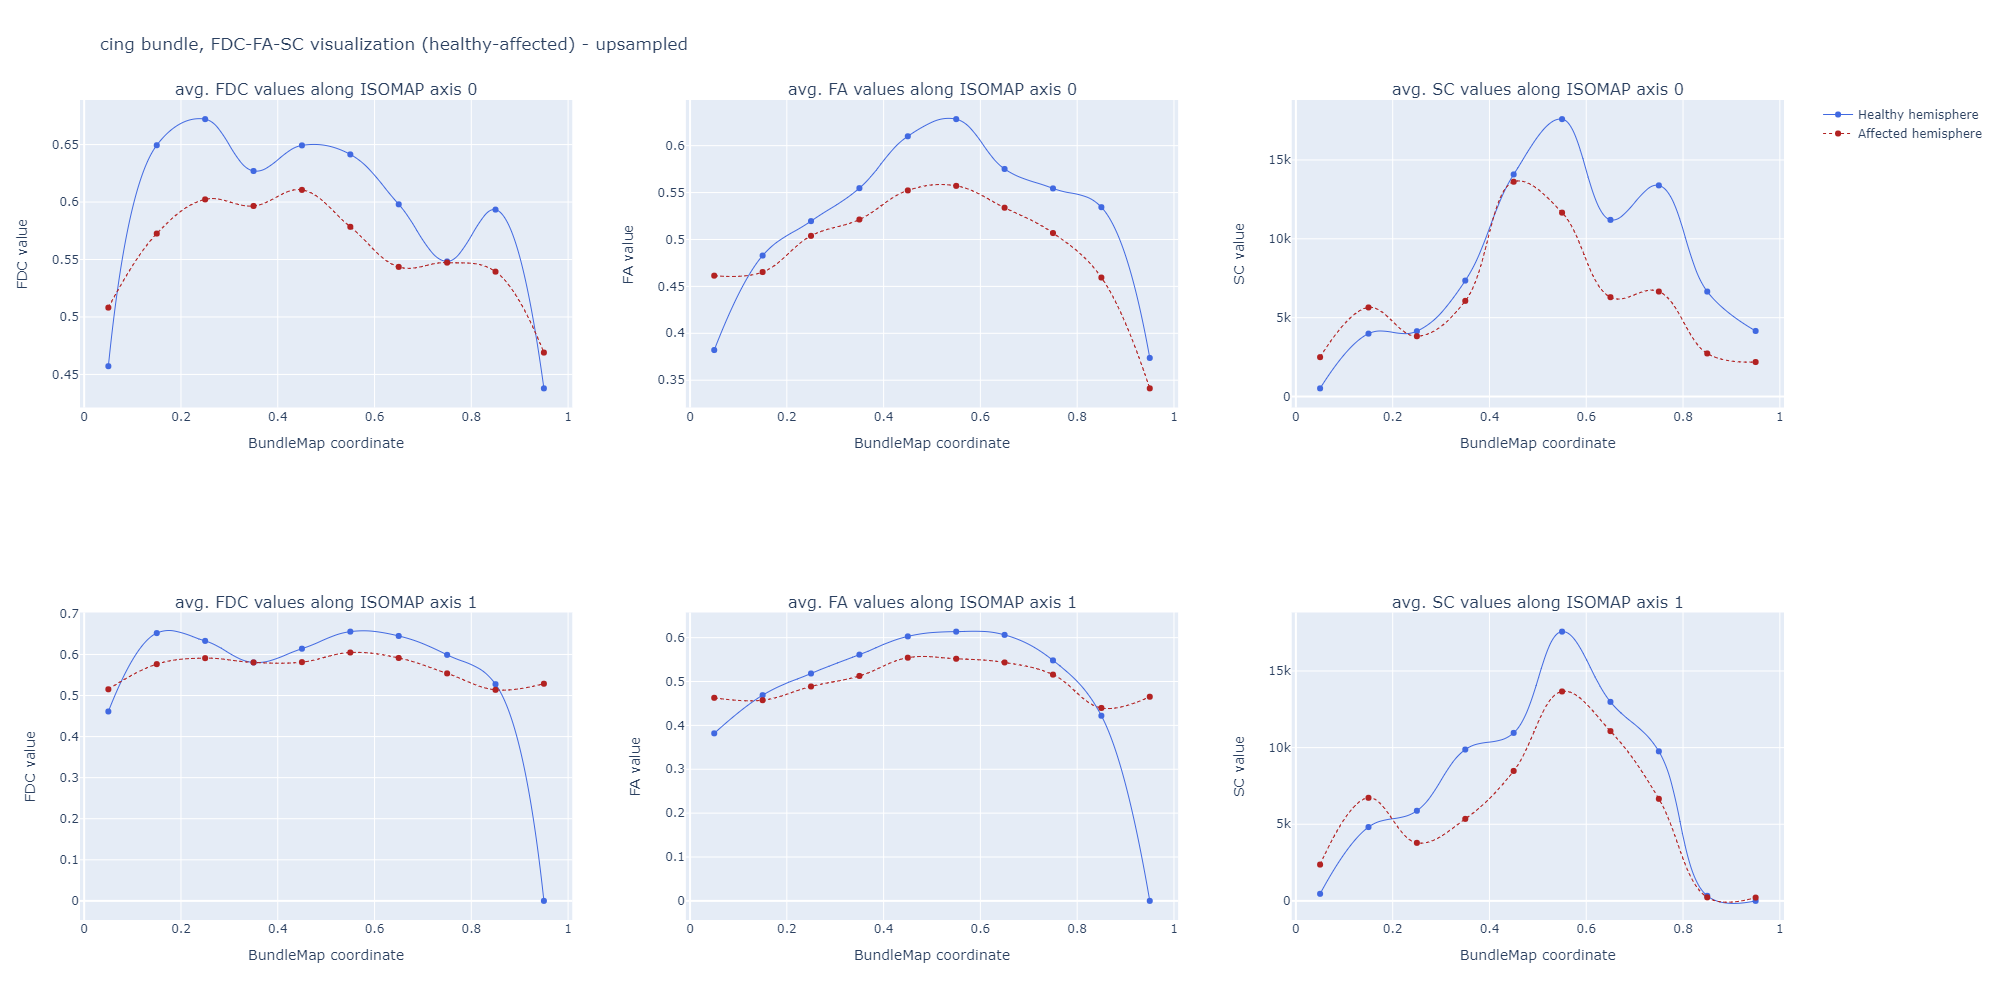
\includegraphics[width=24cm]{thesis_radomskyi/images/cing bundle, FDC-FA-SC visualization (healthy-affected) - upsampled.png}
    \caption{\textbf{Cing Bundle.} FDC-FA-SC visualization (healthy-affected), upsampled.}
    \label{fig:cing-bundle-fdc-fa-sc}
\end{sidewaysfigure}

\begin{sidewaysfigure}
    \centering
  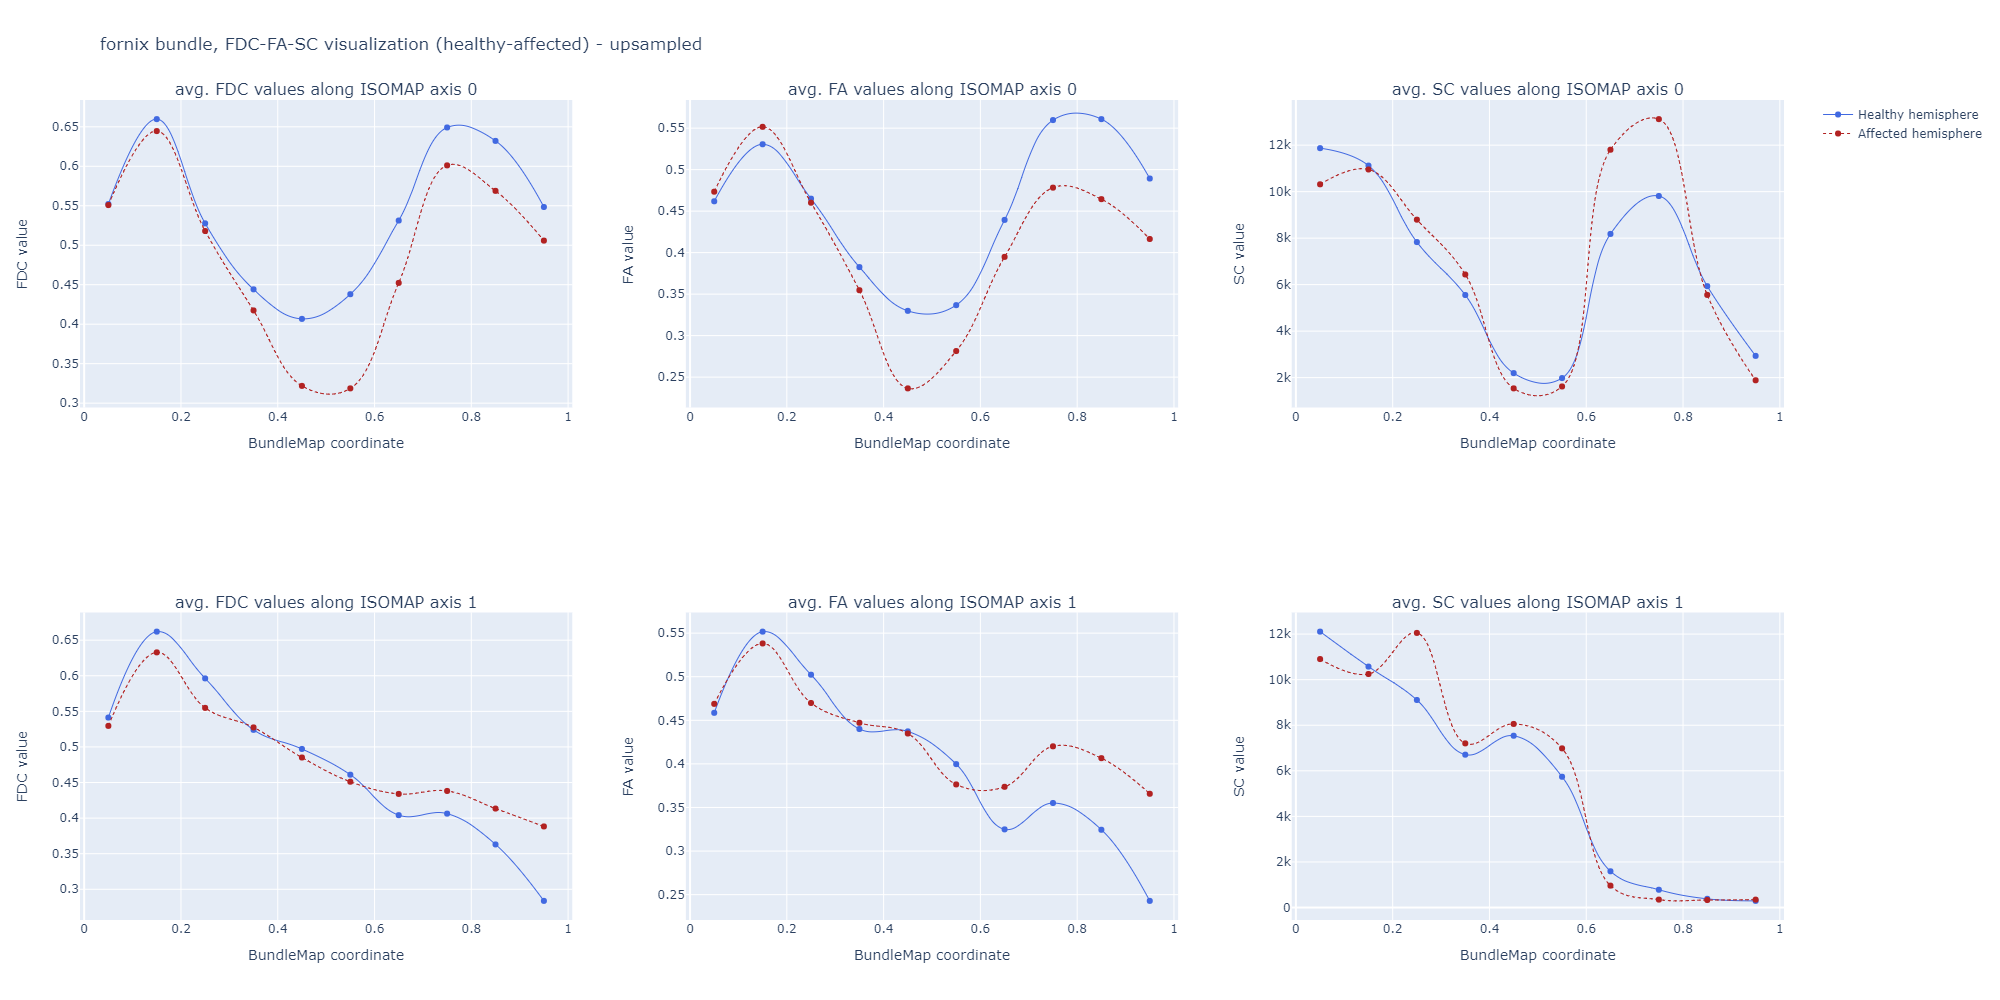
\includegraphics[width=24cm]{thesis_radomskyi/images/fornix bundle, FDC-FA-SC visualization (healthy-affected) - upsampled.png}
    \caption{\textbf{Fornix Bundle.} FDC-FA-SC visualization (healthy-affected), upsampled.}
    \label{fig:fornix-bundle-fdc-fa-sc}
\end{sidewaysfigure}

\begin{sidewaysfigure}
    \centering
  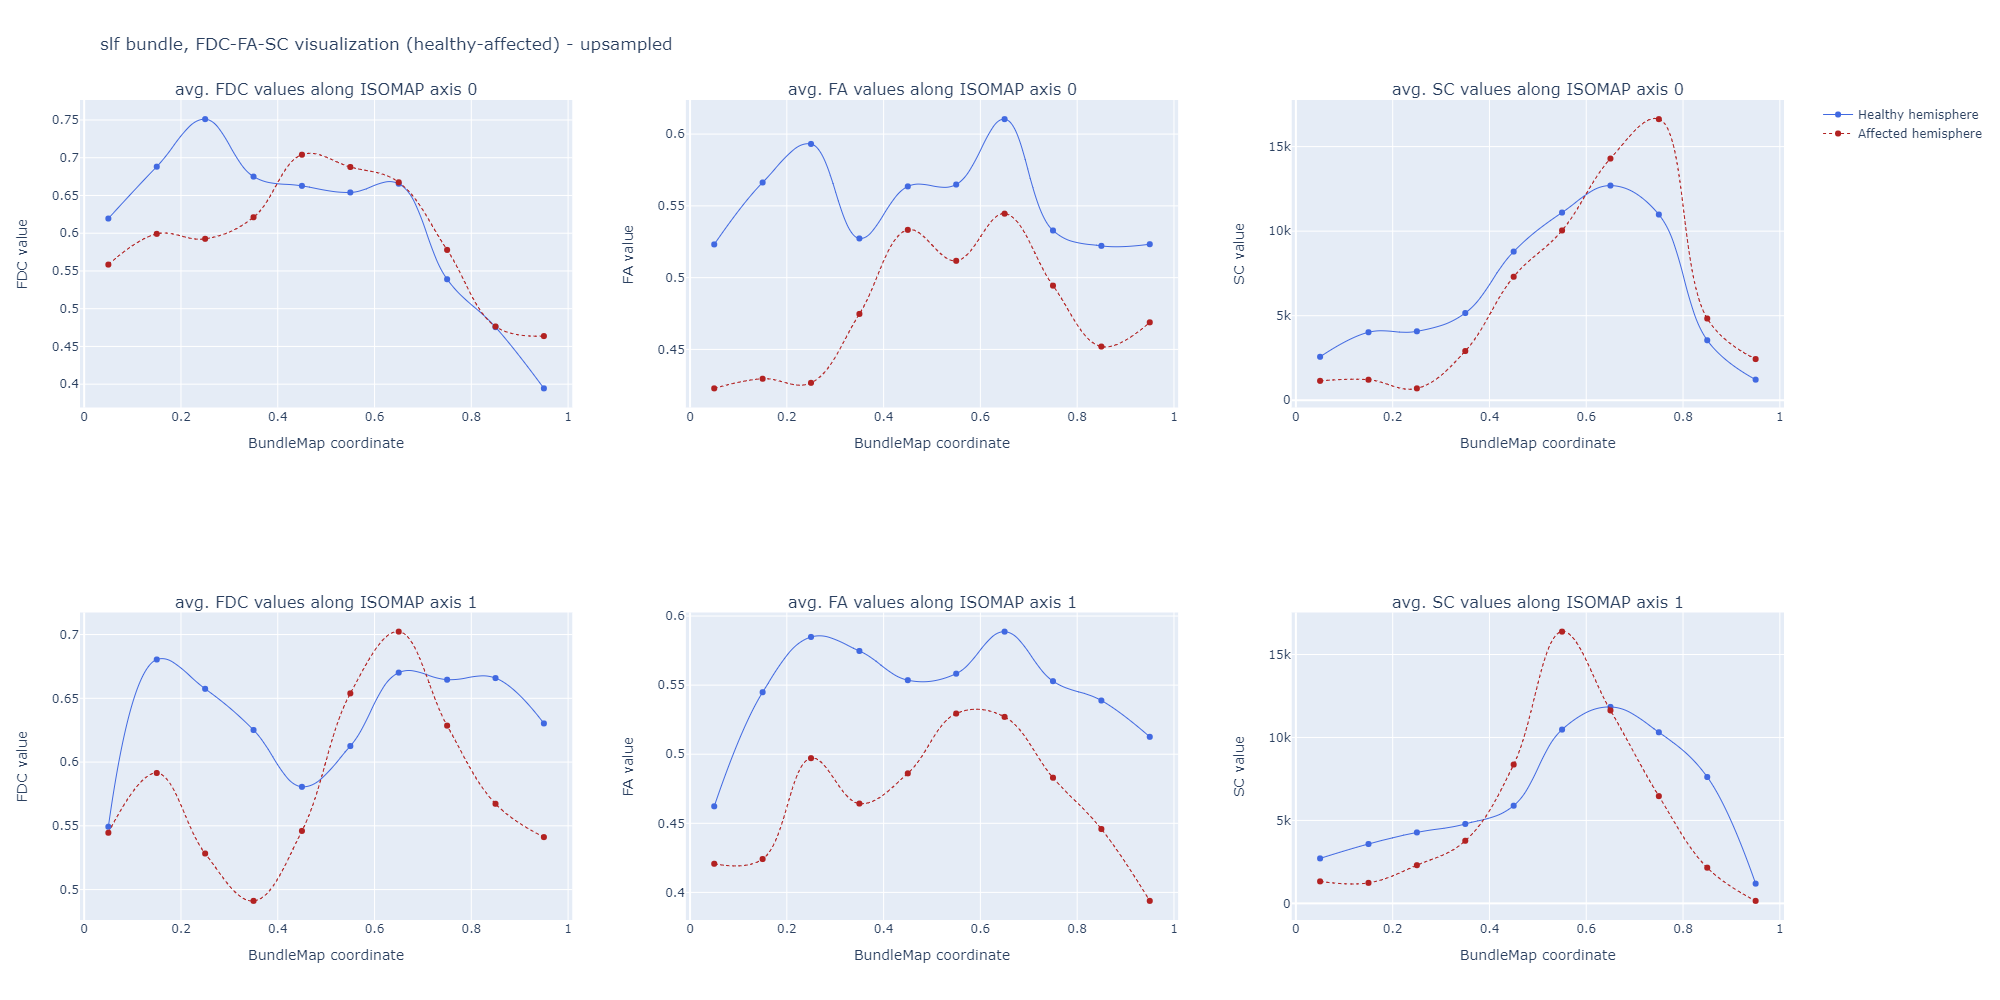
\includegraphics[width=24cm]{thesis_radomskyi/images/slf bundle, FDC-FA-SC visualization (healthy-affected) - upsampled.png}
    \caption{\textbf{SLF Bundle.} FDC-FA-SC visualization (healthy-affected), upsampled.}
    \label{fig:slf-bundle-fdc-fa-sc}
\end{sidewaysfigure}
Figures  \ref{fig:fornix-bundle-fdc-fa-sc}, \ref{fig:cing-bundle-fdc-fa-sc} and \ref{fig:slf-bundle-fdc-fa-sc} depict results of CoBundleMAP parameterization for fornix, cingulum and superior longitudinal fasciculus bundles, presenting ability of visual analysis of extracted FDC, FA and SC measures. Figures \ref{fig:fornix-bundle-fdc-fa-sc} and \ref{fig:cing-bundle-fdc-fa-sc} show the presence of evident correlation between computed FDC and FA values. This is expected and proves the correctness of performed FBA analysis, since both can be interpreted as measures of fiber integrity. The only reason for these metrics to differ is occurrence of glitches, resulting from the presence of crossing fibers. Such errors would affect FA values only, since it is, unlike FDC, very sensitive and error-prone in such areas. Absence of such anomalies can only be explained by robustness of the algorithms and techniques used within CoBundleMAP. Figure \ref{fig:slf-bundle-fdc-fa-sc} is slightly different. Here we can observe a general correspondence between the metrics, though FDC shows slightly less discrepancy between the examined groups along the second half of the CoBundleMAP coordinate. This can be interpreted as a piece of complementing information -- while both metrics show the expected difference, FDC allows to determine the exact bins, where pathology is most prominent. This information can also, in a way, be inferred from FA values, though is not as visually evident.

\subsection{Analysis of FDC-FC-FD correspondence}
\begin{sidewaysfigure}
    \centering
  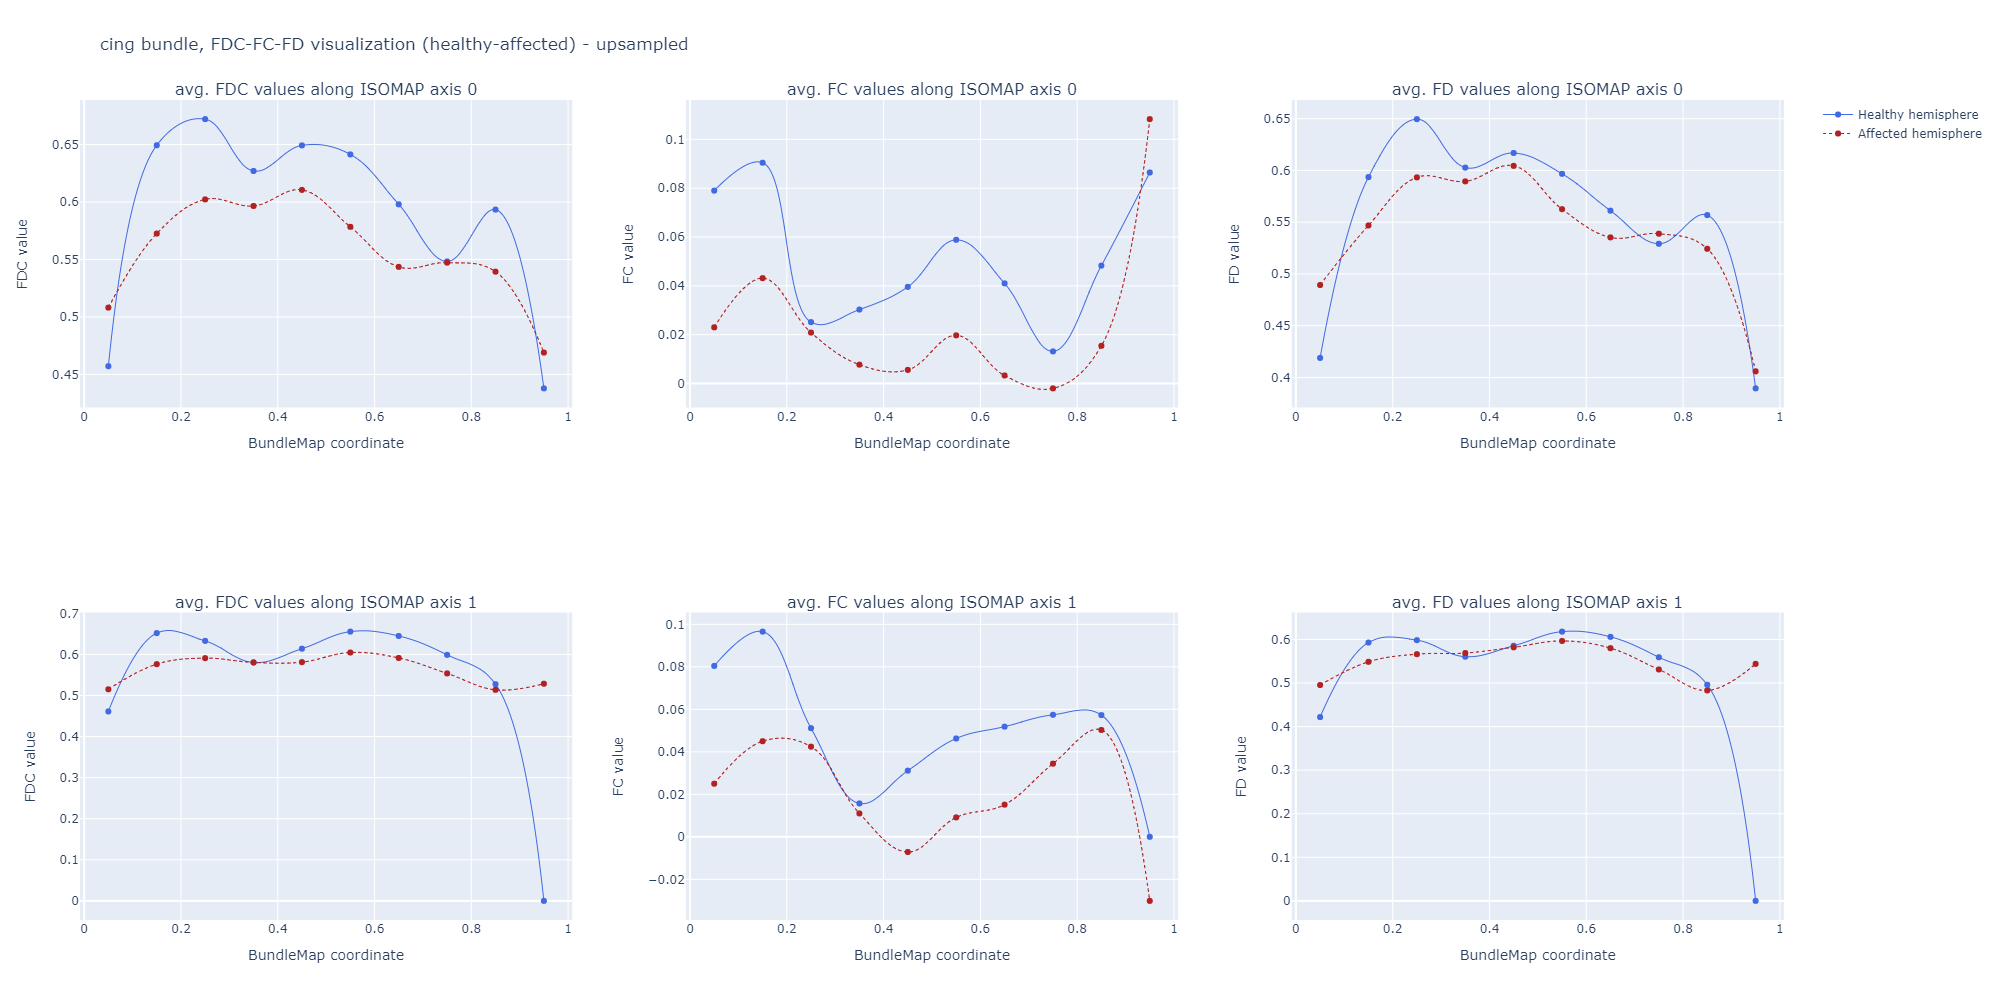
\includegraphics[width=24cm]{thesis_radomskyi/images/cing bundle, FDC-FC-FD visualization (healthy-affected) - upsampled.png}
    \caption{\textbf{Cing Bundle.} FDC-FC-FD visualization (healthy-affected), upsampled.}
    \label{fig:cing-bundle-fdc-fc-fd}
\end{sidewaysfigure}

\begin{sidewaysfigure}
    \centering
  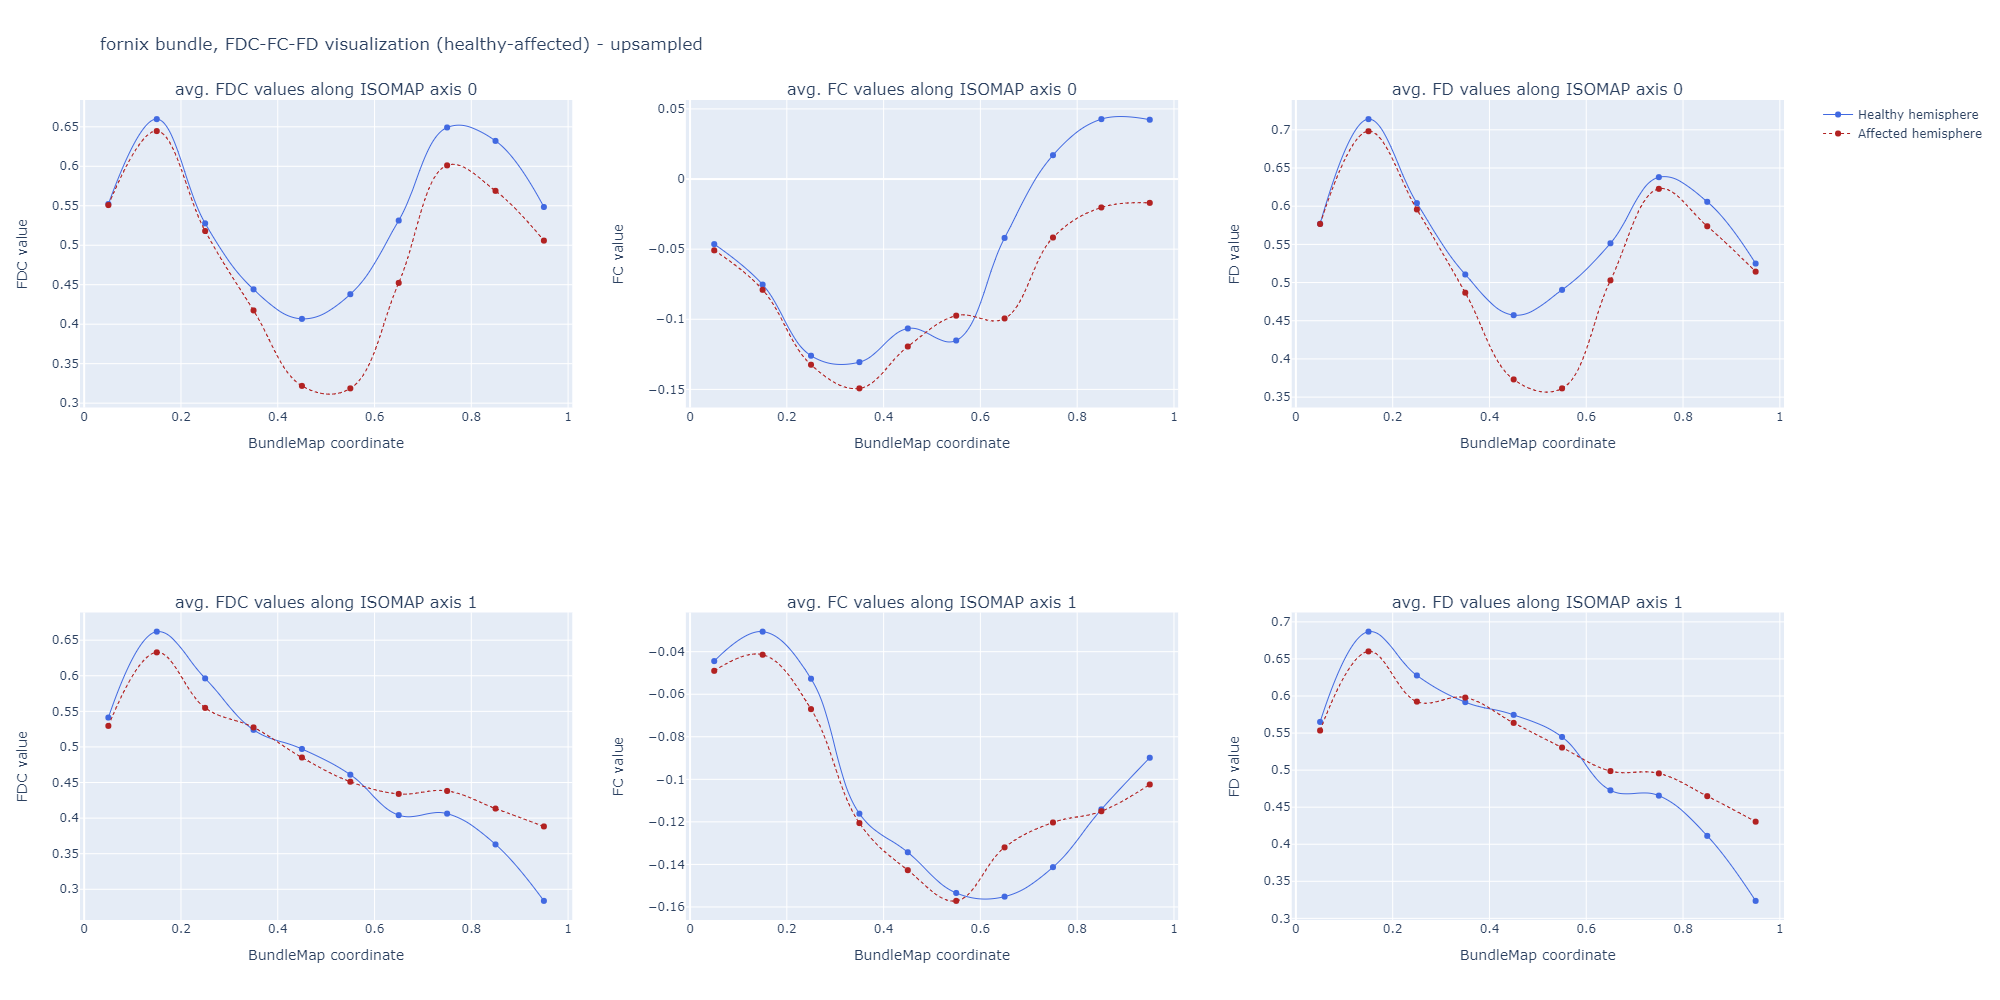
\includegraphics[width=24cm]{thesis_radomskyi/images/fornix bundle, FDC-FC-FD visualization (healthy-affected) - upsampled.png}
    \caption{\textbf{Fornix Bundle.} FDC-FC-FD visualization (healthy-affected), upsampled.}
    \label{fig:fornix-bundle-fdc-fc-fd}
\end{sidewaysfigure}

\begin{sidewaysfigure}
    \centering
  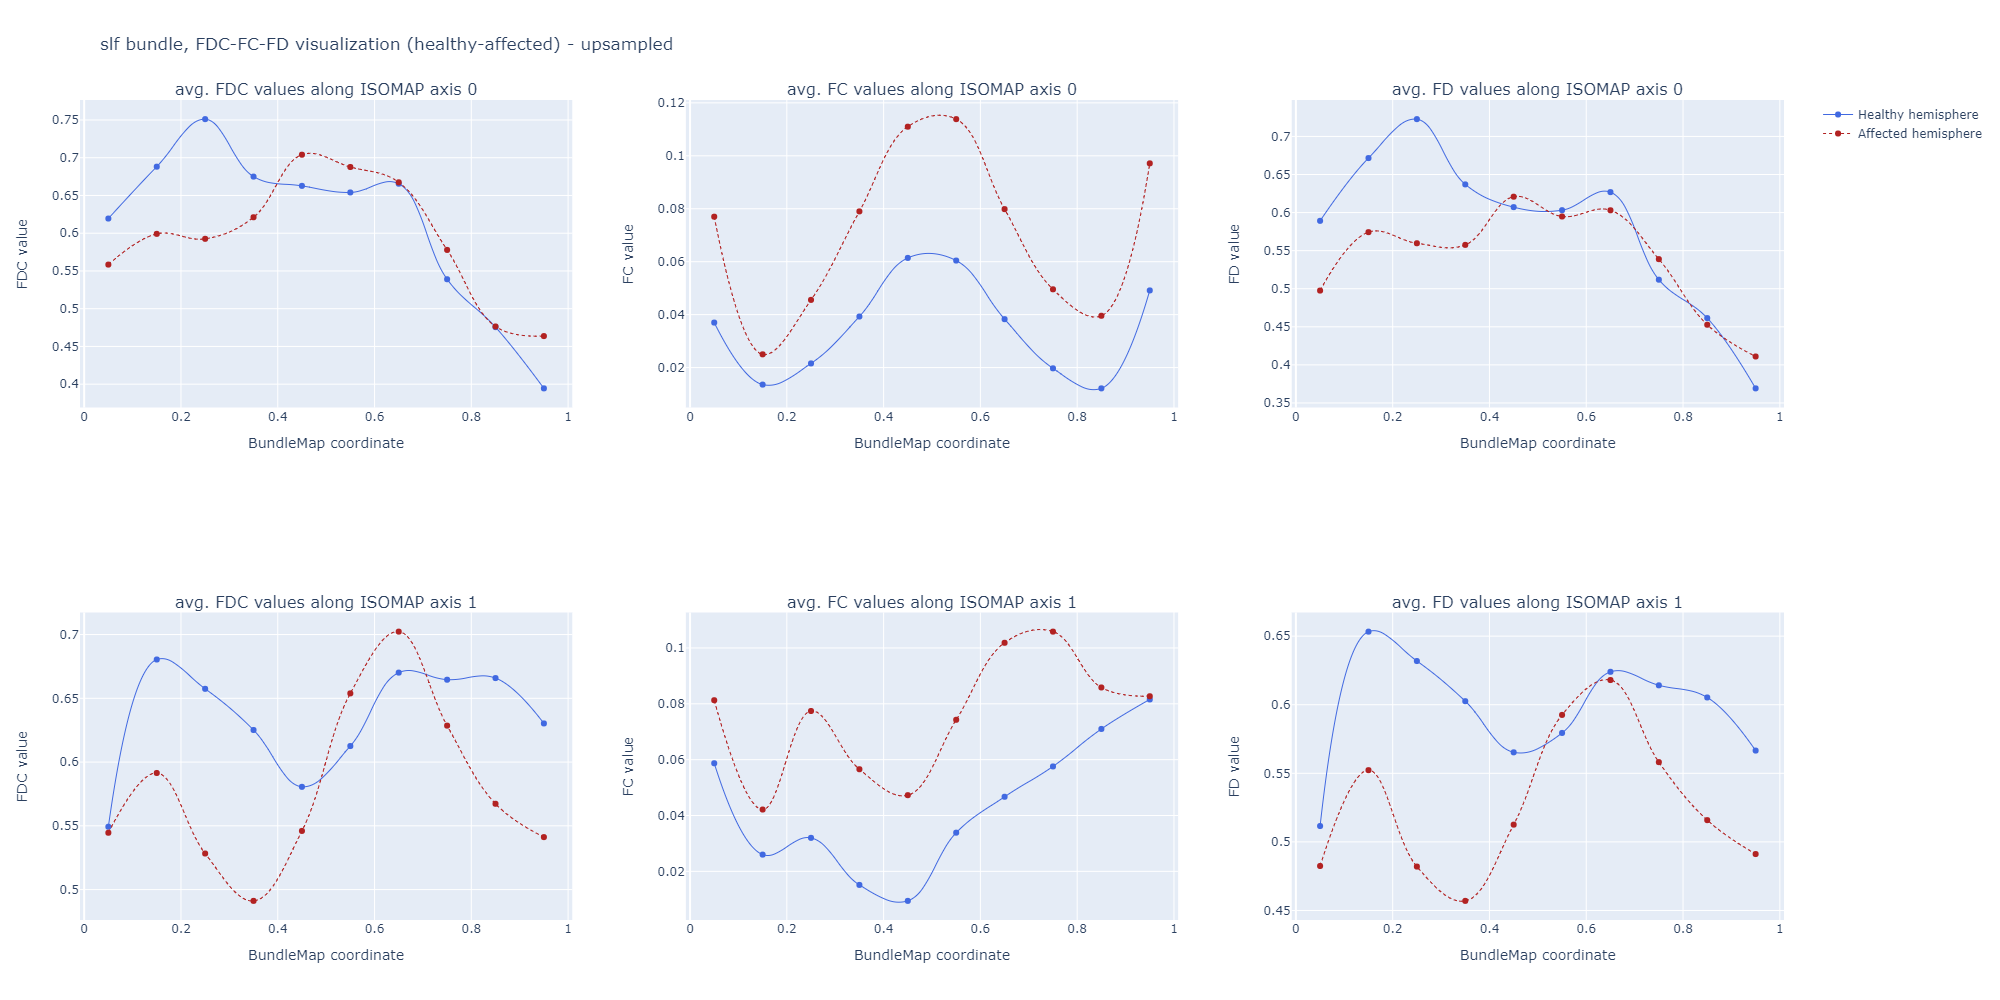
\includegraphics[width=24cm]{thesis_radomskyi/images/slf bundle, FDC-FC-FD visualization (healthy-affected) - upsampled.png}
    \caption{\textbf{SLF Bundle.} FDC-FC-FD visualization (healthy-affected), upsampled.}
    \label{fig:slf-bundle-fdc-fc-fd}
\end{sidewaysfigure}
Next, three more plots will be discussed. They depict all the same bundles, but now contain only FBA-specific metrics, namely FDC, FD and FC. I will analyse what exactly can be inferred from them, and which additional knowledge could be extracted for better understanding of pathologies present within the bundles. The first of three mentioned images, Figure \ref{fig:cing-bundle-fdc-fc-fd} is the visualization of cingulum tract parameterization. It was already concluded that both from the results of FA, as well as FDC computation, this tract shows the presence of noticeable difference between the healthy and affected hemispheres. But presence of two distinct fixel-based values allows to conclude which exact type of pathology is present, and whether such outcome can be considered a pathology at all. By looking at the results of FD and FC extraction, it can be concluded that fiber density stays mostly the same, except for some fluctuations across the first ISOMAP coordinate, within the whole bundle for both groups. A more significant difference is noticeable in fiber cross-section and is present along the most of the bundle in both directions. A conclusion that can be inferred from such observation is that this particular bundle is considerably "thinner" within the affected hemisphere. This may or may not be interpreted as a pathology, but additional insight on the underlying causes is definitely a valuable information, which cannot be acquired through traditional diffusion metrics. Second plot Figure \ref{fig:fornix-bundle-fdc-fc-fd} is depicting fornix white matter tract. Though pathology doesn't seem to be heavy in this case, a conclusion can be made about the exact parts of the bundle which start to exhibit abnormalities. This information can be used for better understanding about the course of disease as well as for early treatment. Last white matter tract that will be discussed within this chapter is superior longitudinal fasciculus (Figure \ref{fig:slf-bundle-fdc-fc-fd}). Even though the presence of pathology was evident from the first plot (Figure \ref{fig:slf-bundle-fdc-fa-sc}), observing the correspondingly aligned FD and FC information allows to conclude that it is more serious than expected. While FDC and FA metrics did show the parts of the bundle that are most affected, comparison of FC and FD gives additional insight about the biological background of observed anomaly. Simultaneous reduction of fiber density accompanied by increase of cross-section is a strong evidence of serious disease, including neuronal loss and gliosis. I believe, this information is of a great value for medical personnel and is something that could not be derived from diffusivity measures alone.

As expected, fixel-derived metrics show a comparable to FA sensitivity for the task of detecting white matter pathologies, though due to high quality of the original images and a well-designed VBA within the CoBundleMAP it was not possible to conclude with definite confidence if it is of great value in areas of crossing fibers. The most important achievement of this combined pipeline is the ability to infer additional information about white matter that are impossible to achieve otherwise.

\end{document}
